\documentclass[10pt,oneside,a4paper]{article}
\usepackage[utf8]{inputenc}
\usepackage{amsmath}
\usepackage{indentfirst}
\usepackage{enumitem}
\usepackage[spanish]{babel}
\usepackage[export]{adjustbox}
\usepackage{graphicx}
\graphicspath{ {img/} }
\usepackage{listings}
\usepackage{subfig}
\usepackage{cite}

\addtolength{\oddsidemargin}{-.300in}
\addtolength{\evensidemargin}{-.300in}
\addtolength{\textwidth}{0.600in}
\addtolength{\topmargin}{-.300in}
\addtolength{\textheight}{0.600in} %1.75

\begin{document}
\begin{titlepage}

\title{\Huge Rendering Avanzado  \\[0.7in] \LARGE Iluminación directa\\[3.6in]}
\date{}
\author{Álvaro Muñoz Fernández\\
Iván Velasco González}
\maketitle
\thispagestyle{empty}
\end{titlepage}

\section{Emmiter Sampling}
En esta parte de la práctica se debía implementar en \textit{nori} todo lo necesario para poder realizar un algoritmo de iluminación directa que muestree directamente las fuentes de luz.
\subsection{Mesh Area Light}
\subsubsection{Triangle Sampling}
El primer paso para poder realizar esta tarea consiste en poder muestrear de forma correcta una malla de triángulos que modelara nuestra fuente de iluminación.\\

En primer lugar, se implementó un método \textit{sampleTriangle()} que obtiene la posición y la normal de un punto interno al triángulo a partir de un sample 2D que se emplea, por medio de la conversión de distribuciones, como coordenadas baricéntricas del triángulo. Sin embargo, esto nos proporciona únicamente dos coordenadas baricéntricas, pero a partir de $ u + v + w = 1$, la última coordenada se obtiene como $ w = 1 - u - v$. Una vez obtenidas todas las coordenadas baricéntricas se interpola la posición del punto a partir de la posición de los vértices que componen el triangulo, y se realiza un proceso similar para calcular su normal. Es importante destacar que, en caso de que las mallas que conforman las luces no tengan normales asociadas, el algoritmo dará un error al intentar acceder a estas normales.\\

Una vez podemos muestrear un triángulo de forma correcta, es necesario elegir que triángulo de toda la malla se ha de escoger para ser muestreado, teniendo en cuenta que la probabilidad de que un triángulo sea muestreado debe ser proporcional al área que tenga este respecto a la malla completa. Para conseguir esta PDF se ha utilizado la clase \textit{DiscretePDF} implementada por \textit{nori}, la cual se ha inicializado añadiéndole el área de todos los triángulos en su orden de aparición en la malla, y después se ha normalizado. Una vez tenemos construida esta PDF, para muestrear un triángulo simplemente se le pide una muestra a esta distribución a partir de un nuevo valor aleatorio, distinto que los usados para muestrear el triángulo en sí, para evitar correlar \textit{samples}.\\

Por último, para calcular la pdf del punto concreto respecto a todo la malla, simplemente se devuelve la inversa del área de la malla, ya que el método de muestreo es uniforme.
\subsubsection{Area Emitter}
En esta parte de la practica se debían rellenar todos los métodos necesarios para poder utilizar una luz de área en un integrador. Para ello, se han aprovechado los métodos de muestreo implementados en el apartado anterior. Los  métodos a implementar para poder utilizar estas luces de área en un integrador son: \textit{sample} \textit{eval} y \textit{pdf}.\\

En primer lugar, se debe tener en cuenta que todos los métodos de esta clase reciben como entrada un \textit{EmitterQueryRecord} el cual es el encargado de almacenar toda la información necesaria para que los métodos de la clase funcionen correctamente.\\

Seguidamente se detallará la implementación del método \textit{sample}. Este método es el encargado de, a partir del punto a iluminar y una muestra, muestrear un punto de la fuente de luz y rellenar todo el \textit{EmitterQueryRecord} de forma consecuente, teniendo en cuenta el punto a iluminar y el punto de la fuente de luz sampleado. En primer lugar, se rellena el registro con: el punto muestreado y su normal, los cuales son obtenidos por medio de una llamada al método de muestreo de la malla implementado en el apartado anterior y la \textit{PDF} del punto sampleado. Además, también se rellena la distancia entre el punto a iluminar y el punto sampleado en la fuente de luz, y el vector incidente desde el punto a iluminar a la fuente de luz.\\

Respecto al método \textit{eval}, este es el encargado de, a partir de un \textit{EmitterQueryRecord} rellenado de forma correcta, por la función de muestreo o por otro método, devolver la luz que recibe el punto a iluminar desde el punto de la luz elegido. Teniendo en cuenta que no es necesario realizar ningún \textit{test} de oclusión en esta evaluación, ya que de esto se encargará el integrador, se comprueba si el rayo incidente a la luz procede de la cara trasera del triángulo, ya que en este caso la iluminación devuelta debería ser 0. Esto se comprueba por medio del producto escalar entre el rayo incidente y la normal, siendo que si este es mayor que 0 el rayo procede de la cara trasera del triángulo. En caso de que esto no sea así y el rayo proceda de la cara delantera del triángulo, la iluminación que recibe el punto a iluminar del punto sampleado será la radiancia atenuada por la distancia, es decir, $Radiance_p = \frac{Radiance}{Distance^2}$\\

Por último, sería necesario implementar el método \textit{pdf()}, el cual debe devolver la PDF del punto sampleado respecto a ángulo sólido. Sin embargo, en el \textit{EmitterQueryRecord} la PDF viene expresada respecto del área, ya que es la forma en la que se ha calculado en la malla que representa la fuente de iluminación. Por lo tanto, para obtener la PDF expresada en ángulo sólido a partir de la PDF expresada respecto al área se ha usado la expresión $p_\Omega(x,xl) = p_S(xl)\frac{||x-xl||^2}{nl\cdot\omega_i}$.\\

\subsection{Integrator}
En esta parte de la práctica se debía implementar un método de iluminación directa, es decir, un integrador de \textit{nori} a partir de la siguiente expresión se iluminación:
$$L_o = Le(x,\omega_o) + \int_\Omega Li(x,\omega_i) * brdf(x,\omega_o,\omega_i)  * \cos\theta_i d\omega_i$$
Teniendo en cuenta que las direcciones de los rayos incidentes ($\omega_i$) van a ser calculadas por medio de un muestreo de las fuentes de luz de la escena.\\

Para realizar esto, en un primer lugar se trazará el rayo de cámara y se comprobará si colisiona o no con la geometría de la escena. En caso de que colisione, se obtienen el punto de la colisión y su normal asociada. Seguidamente comprobamos si el punto a iluminar pertenece a una fuente de luz. Si esto es así se construye un \textit{EmitterQueryRecord}, donde la dirección de incidencia a la luz es igual a la dirección del rayo de cámara y su distancia se ha fijado proxima a 0, y no 0, para evitar errores de calculo.\\

En el caso de que el rayo de la cámara no interseque con una fuente de luz, pero sí con algún elemento de la escena, se muestreará un punto de iluminación de la escena. Para ello se ha usado la función \textit{sampleEmitter} implementada por \textit{nori}, quel nos devuelve una fuente de luz de la escena y su \textit{PDF} asociada. Seguidamente se realiza el muestreo de un punto concreto de esta fuente de luz obteniendo un \textit{EmitterQueryRecord} que encapsula toda la información del muestreo.\\

Seguidamente se rellena un \textit{BSDFQueryRecord} con los datos obtenidos del muestreo de la luz para obtener el valor de la \textit{BRDF} en ese punto. Para ello se rellena con el rayo incidente y saliente, dados por el rayo de cámara y el rayo a la fuente de iluminación respectivamente, teniendo en cuenta que ambos deben estar en coordenadas locales al punto a iluminar.\\

Después debido a que el punto de la fuente de luz ha sido muestreado, es necesario comprobar si el punto a iluminar y el punto de la fuente de iluminación tienen visibilidad entre si, para ello se traza un rayo de sombra en la dirección que une los dos puntos y se comprueba si el rayo interseca con la luz, si esto es así los puntos son visibles entre ellos y no lo serán en caso contrario.\\

Por ultimo, con toda la información necesaria calculada se procede a calcular la iluminación total en el punto a iluminar aplicando la siguiente expresión, la cual es el estimador de Monte Carlo de la función de iluminación vista al principio de esta sección, teniendo en cuenta que luego \textit{nori} sumará y ponderará las muestras:
 $$L_o = L_e  + \frac{ V * L_i * brdf * \cos{\theta}}{P_{light} * P_{point}}$$ 
Donde $Le$ hace referencia a la luz emitida, por lo que solo tendrá valor en las fuentes de luz; $V$ hace referencia a la visibilidad entre el punto a iluminar y la fuente de luz, lo cual es necesario tener en cuenta debido a que el punto de la fuente de luz se ha escogido mediante un muestreio y, por tanto, podría estar ocluido; $Li$ representa la cantidad total de luz incidente, que será la luz directa de las fuentes de luz al tratarse de un método de iluminación directa; y $P_{light}$ y $P_{point}$ hacen referencia a la \textit{PDF} de la fuente de luz escogida y a la \textit{PDF} del punto respecto a esa fuente de luz respectivamente.

\begin{figure}[h]
\centering
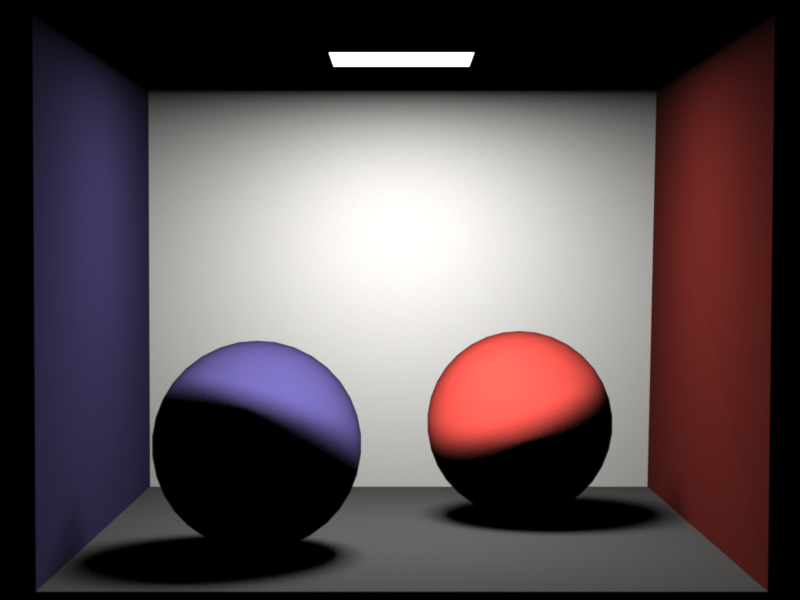
\includegraphics[width=.6\linewidth]{images/cbox_direct_ems_diff_512.png}
\caption{Imagen generada con iluminación directa muestreando las fuentes de luz}
\label{fig:disp}
\end{figure} 
\subsection{BRDF Sampling}
En esta parte de la practica se debía implementar un método de iluminación directa muy similar al propuesto en el apartado anterior, con la salvedad de que la dirección de los rayos incidentes debían calcularse atendiendo a la \textit{BRDF} del material.\\

Por lo tanto la primera parte del proceso es similar. En primer lugar se obtienen el punto al iluminar y su respectiva normal y se comprueba si el punto pertenece a un emisor. Sin embargo, ahora para calcular la dirección del nuevo rayo se utiliza la función \textit{sample} de la clase \textit{BSDF} para obtener un \textit{BSDFQueryRecord} que contiene toda la información relativa al muestreo de esa \textit{BSDF} en concreto, como la orientación del rayo de salida, la pdf de la dirección dada y, por supuesto, el valor en si de la \textit{BRDF} asociado a las dos direcciones.\\

Una vez obtenido el muestreo de la BRDF se traza un rayo en la dirección obtenida y se comprueba si interseca con una fuente de luz. Si lo hace se rellena un \textit{EmitterQueryRecord} con todos los datos necesarios y se evalúa la cantidad de iluminación que recibe el punto proveniente de esa fuente de luz. En el caso de que el rayo no interseque con una fuente de luz la iluminación recibida por el punto será 0 si interseca con geometría, o la intensidad de luz proveniente del fondo si no interseca con nada. Esto afectará de forma negativa a la convergencia como se verá en otro apartado.\\

Seguidamente, una vez tenemos todos los valores necesarios se calcula la siguiente expresión, teniendo en cuenta, como en el caso anterior, que \textit{nori} fusionará estas muestras:
$$L_o = L_e + \frac{Li * brdf *\cos\theta}{P_{dir}}$$
Donde $P_{dir}$ hace referencia a la \textit{PDF} del rayo generado por la función de sampleo de la BRDF en el punto a iluminar. Nótese que, al contrario que en el apartado anterior, no tenemos el término de visibilidad ($V$) debido a que en el caso anterior el punto de la fuente de luz era obtenido mediante muestreo (pudiendo estar ocluido), y en este caso el punto de luz se ha obtenido como la intersección de un rayo con la geometría de la escena (no pudiendo estar ocluido).\\

Por último es necesario tener una serie de consideraciones respecto a la implementación. En \textit{nori} las \textit{BRDF} discretas devuelven un valor de 0 tanto en la \textit{BRDF} como en la \textit{PDF}, esto provocaba que los brillos especulares de un espejo no se vieran ya que evaluaban a 0 la función de iluminación. Para solucionarlo se ha comprobado si la \textit{PDF} es de tipo discreto y se han asignado tanto al color como a la \textit{PDF} un valor de 1. Por otro lado, nos hemos encontrado el problema que al muestrear la BRDF, a veces el rayo incidente procedía de la parte trasera del triángulo con el que intersecaba. Suponemos que debido a problemas de precisión, devolviendo 0 tanto la \textit{PDF} como la \textit{BRDF}. Por lo tanto, para solucionarlo se tienen en cuenta estas circunstancias y si la \textit{PDF} devuelta por un muestreo de la \textit{BRDF}, que no sea de tipo discreta, tiene valor 0 se devuelve una $L_o$ de 0 sin tener en cuenta la ecuación, para evitar errores de cálculo. Un ejemplo de estos puntos puede verse en la figura \ref{fig:diff_ems}.

\begin{figure}[h]
\centering
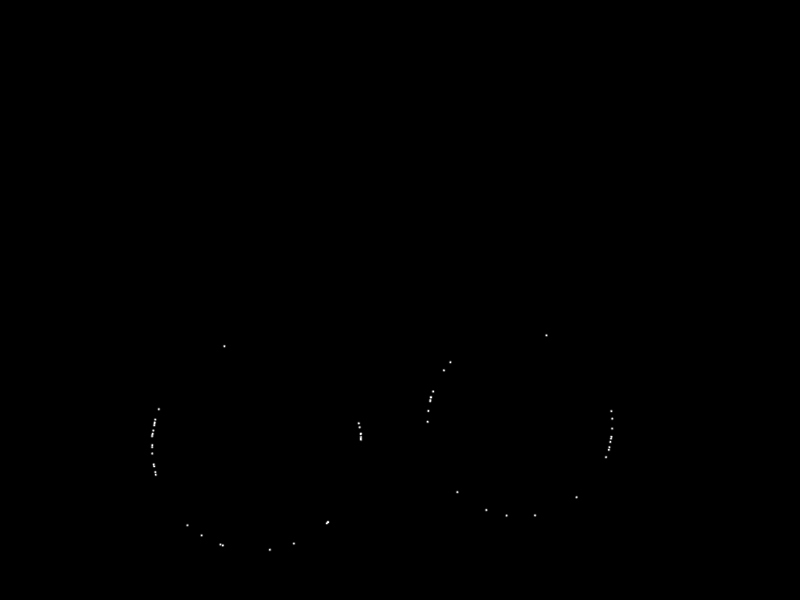
\includegraphics[width=.6\linewidth]{images/pdfs_incorrectas.png}
\caption{Puntos que causan PDFs incorrectas}
\label{fig:diff_ems}
\end{figure}

\begin{figure}[h]
\centering
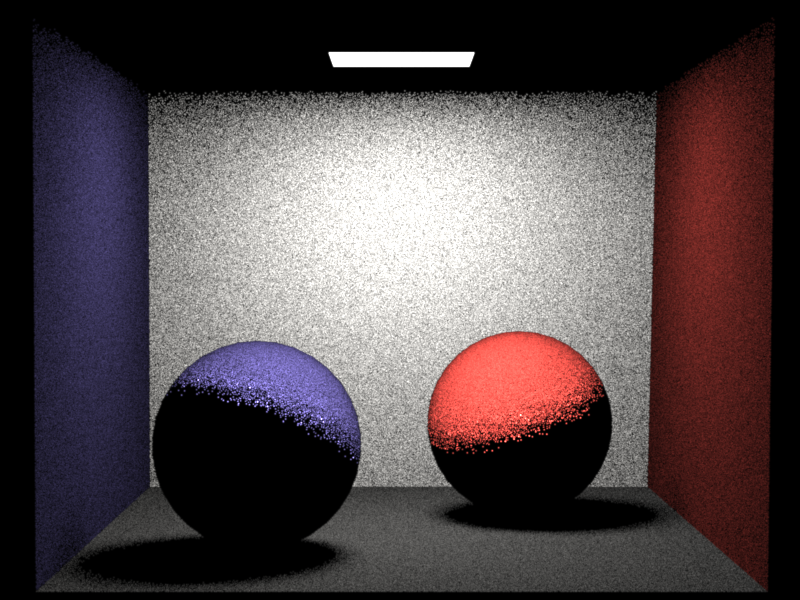
\includegraphics[width=.6\linewidth]{images/cbox_direct_mats_diff_512.png}
\caption{Imagen generada con iluminación directa muestreando la BRDF}
\label{fig:disp}
\end{figure}


\subsection{Dielectric}
En esta parte de la práctica se debía implementar un material dieléctrico ideal, por lo tanto, se tratará de una BRDF determinista ya que para un rayo incidente siempre le corresponderá el mismo rayo de salida. Ademas se debe tener en cuenta que este tipo de BRDF es de tipo discreta en \textit{nori}.\\

En primer lugar, a partir del rayo incidente y de los coeficientes de reflexión de los medios calculamos el término de \textit{fresnel}, utilizando para ello la función \textit{fresnel} implementada por \textit{nori}. Una vez hemos hallado este coeficiente que determina la probabilidad de que un rayo incidente sea reflejado o transmitido, se compara con un valor aleatorio para decidir si se trazara el rayo reflejado o el transmitido. En el caso de que se deba trazar el rayo reflejado su dirección será calculada invirtiendo el signo de las componentes $x$ e $y$ del rayo incidente, ya que ambos rayos se encuentran expresados en coordenadas locales al punto a iluminar con la normal de la superficie apuntando al exterior. En caso de que el rayo a trazar sea el transmitido se calcula el ángulo de salida ($\theta_t$) de este, de un modo similar al utilizado por la función \textit{fresnel}. Seguidamente, a partir de este ángulo de salida($\theta_t$) se calcula la dirección del rayo saliente como
 $ w_o = (-\frac{n1}{n2},-\frac{n1}{n2},\cos\theta_t)$. Esto, al igual que en el caso anterior, se debe a que ambos rayos están expresados en coordenadas locales al punto, con la normal apuntando a $(0,0,1)$ y, por lo tanto, $\cos\theta$ corresponde con la coordenada $z$.\\
 
Ademas hay que tener en cuenta que se han realizado varias comprobaciones para capturar las casuísticas de que el rayo proceda del exterior, o por el contrario proceda de la parte interna del material. Esto en un caso de luz directa no tiene importancia, ya que si un rayo entra en el interior del objeto no podrá salir nunca al haber solo un rebote, por lo que solamente puede darse el caso de rayos que pasen del medio al material. Sin embargo tendrá una gran importancia en el \textit{Path Tracer}, donde sí pueden darse estos rebotes de dentro del material al exterior.
 
 \begin{figure}[h]
\centering
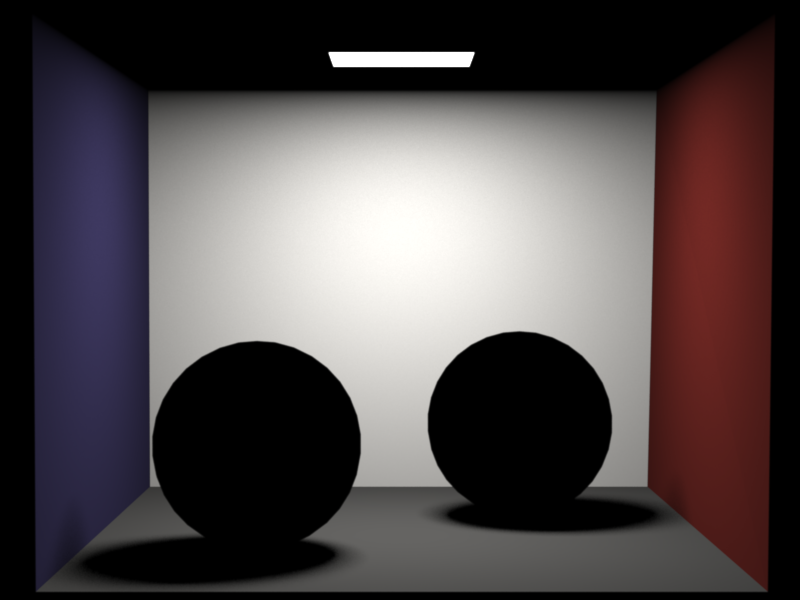
\includegraphics[width=.6\linewidth]{images/cbox_direct_ems_comlex_512.png}
\caption{Imagen generada con iluminacion directa muestreando las fuentes de luz}
\label{fig:disp}
\end{figure}

\begin{figure}[h]
\centering
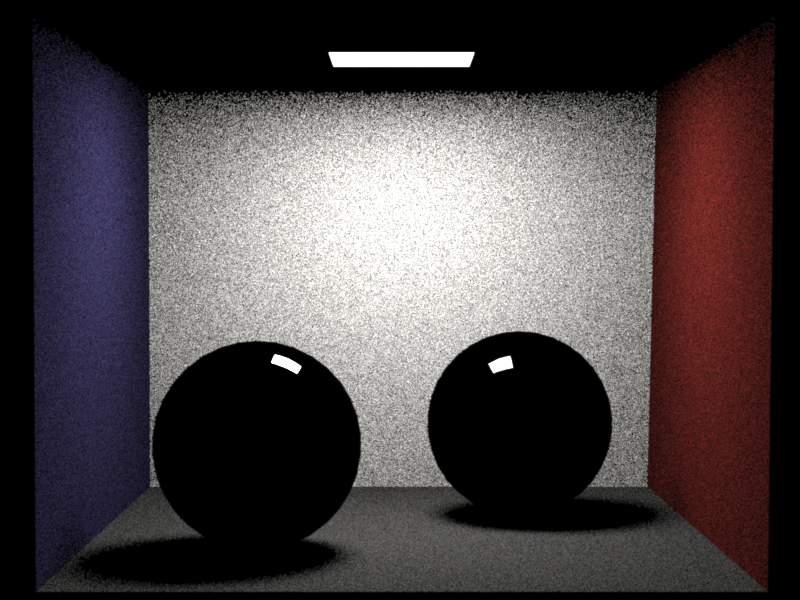
\includegraphics[width=.6\linewidth]{images/cbox_direct_mats_complex_512.png}
\caption{Imagen generada con iluminacion directa muestreando la BRDF}
\label{fig:disp}
\end{figure}

 
 \subsection{Discussion}
 En esta sección se van a discutir las diferencias encontradas respescto a los dos métodos de iluminación directa implementados, por un lado respecto al sampleo de las fuentes de luz de la escena y por el otro respecto al muestreo de la \textit{BRDF}.\\
 
 En ambos casos, se puede observar cómo para materiales difusos ambas se comportan de una forma similar, sin embargo muestrear las fuentes de luz consigue una mejor convergencia para el mismo número de muestras que muestreando la \textit{BRDF} de los materiales. Esto se debe a que al muestrear la \textit{BRDF} es posible que algunas muestras no caigan en la fuente de luz, y como solo hay un rebote la contribución de esa muestra sea 0, desperdiciándose estas muestras. Por lo tanto, este método funciona mejor mientras mayor área tengan las luces en la escena ya que será mas probable que sean muestreadas.\\
 
Sin embargo, cuando añadimos materiales más complejos como espejos o dieléctricos, nos encontramos con que muestreando las fuentes de luz no conseguimos capturar efectos como los reflejos o la transmisión. Debido principalmente a que, como estos materiales son de tipo discreto en \textit{nori}, siempre devolverá un valor de 0 tanto su \textit{BRDF} como su \textit{PDF}.\\
 
 \subsection{Interesting Image}
 En esta sección se ha diseñado una imagen que, junto con las otras, muestra las limitaciones de la iluminación directa. Además también muestra algunos efectos en el dieléctrico y en los espejos que no se han podido visualizar previamente. Por lo tanto, se ha usado el metodo basado en la BRDF para renderizar\\
 
 \begin{figure}[h]
\centering
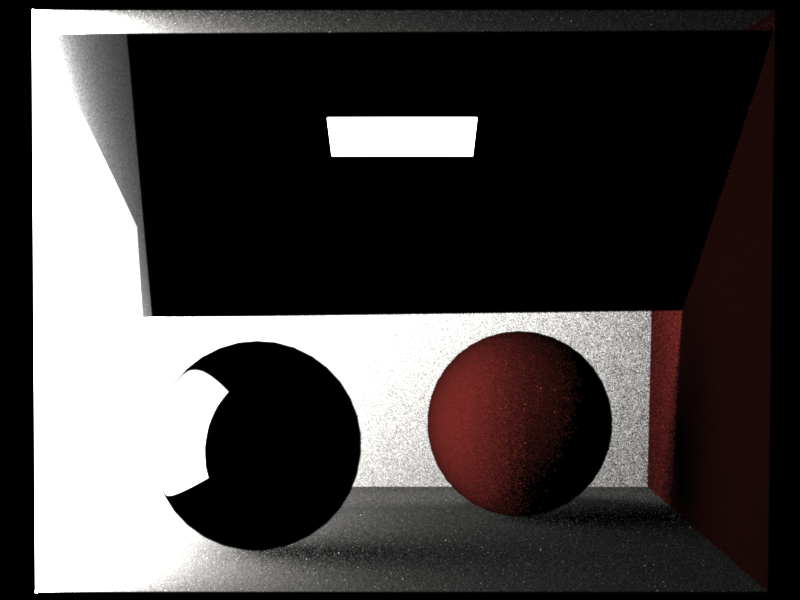
\includegraphics[width=.6\linewidth]{images/cbox_interesting_512.png}
\caption{Imagen donde pueden verse algunos de los efectos que se pueden conseguir}
\label{fig:disp}
\end{figure}
 
 Como puede observarse en la imagen podemos observar cómo el reflejo producido en la esfera solamente tiene en cuenta la luz procedente de la pared derecha, esto se debe a que la luz del techo se encuentra ocluida por un cristal (un dieléctrico) y aunque este deje pasar los rayos de luz, al tener solamente un único rebote no se trazará nunca el rayo transmitido partiendo del reflejo creado por la esfera. Por otro lado, podemos observar cómo en el caso del cristal, el cual es el plano inclinado, sí que se muestran ambas luces, debido a que los rayos incidentes en él sí que son refractados. Además también puede observarse cómo este cristal redirige la orientación de los rayos en la esquina que forma respecto a la pared luminosa.
 
  

\end{document}